\documentclass[a4paper]{article}

\input{../latex_template/style/ch_xelatex.tex}

\lstset{numbers=left,
basicstyle=\tiny,
numberstyle=\tiny,
keywordstyle=\color{blue!70},
commentstyle=\color{red!50!green!50!blue!50},
frame=single, rulesepcolor=\color{red!20!green!20!blue!20},
escapeinside=``
}

\graphicspath{ {./figures/} }
\usepackage{ctex}
\usepackage{graphicx}
\usepackage{color,framed}
\usepackage{listings}
\usepackage{caption}
\usepackage{amssymb}
\usepackage{enumerate}
\usepackage{xcolor}
\usepackage{bm}
\usepackage{lastpage}
\usepackage{fancyhdr}
\usepackage{tabularx}
\usepackage{geometry}
\usepackage{graphics}
\usepackage{subfigure}
\usepackage{float}
\usepackage{multirow}
\usepackage{booktabs}

\usepackage{algorithm}
\usepackage{algorithmicx}
\usepackage{algpseudocode}
\floatname{algorithm}{Algorithm}
\renewcommand{\algorithmicrequire}{\textbf{Input:}}
\renewcommand{\algorithmicensure}{\textbf{Output:}}

\geometry{a4paper,left=2.3cm,right=2.3cm,top=2.7cm,bottom=2.7cm}
\usepackage{fancyhdr}
\pagestyle{fancy}
\lhead{\kaishu \leftmark}
\rhead{\kaishu 并行程序设计实验报告}
\lfoot{}
\cfoot{\thepage}
\rfoot{}
\renewcommand{\headrulewidth}{0.1pt}
\renewcommand{\footrulewidth}{0pt}
\setlength{\textfloatsep}{10mm}

\begin{document}
\renewcommand{\contentsname}{目\ 录}
\renewcommand{\refname}{参考文献}
\renewcommand{\figurename}{图}
\renewcommand{\tablename}{表}
\renewcommand{\today}{\number\year 年 \number\month 月 \number\day 日}

%-------------------------封面----------------
\begin{titlepage}
    \begin{center}
    
\includegraphics[width=0.8\textwidth]{../latex_template/NKU.png}\\[1cm]
    \vspace{20mm}
        \textbf{\huge\textbf{\kaishu{计算机学院}}}\\[0.5cm]
        \textbf{\huge{\kaishu{并行程序设计报告}}}\\[2.3cm]
        \textbf{\Huge\textbf{\kaishu{MPI 多进程加速}}}\\[0.3cm]
        \textbf{\Huge\textbf{\kaishu{的高斯消去算法}}}

        \vspace{\fill}
    \centering
    \textsc{\LARGE \kaishu{姓名\ :\ 王毅豪}}\\[0.5cm]
    \textsc{\LARGE \kaishu{学号\ :\ 2412509}}\\[0.5cm]
    \textsc{\LARGE \kaishu{专业\ :\ 计算机科学与技术}}\\[0.5cm]

    \vfill
    {\Large \today}
    \end{center}
\end{titlepage}

\renewcommand {\thefigure}{\thesection{}.\arabic{figure}}
\renewcommand{\figurename}{图}
\renewcommand{\contentsname}{目录}
\cfoot{\thepage\ of \pageref{LastPage}}

% 目录
\clearpage
\tableofcontents
\newpage

%============================ 正文 ============================

\section{实验目标与问题描述}

本次实验的目标是在 ARM 架构平台（华为鲲鹏 920 集群）上，使用 MPI（Message Passing Interface）多进程编程模型，对普通高斯消去算法进行分布式并行化优化。

\subsection{从多线程到多进程}

在前三次实验中，我们逐步完成了从串行到单核 SIMD 再到单节点多线程的性能优化：Lab2 通过 NEON SIMD 向量化获得了约 2.0x 的单核加速比；Lab3 通过 Pthread 和 OpenMP 多线程分别获得了最高 4.12x 和 9.64x 的单节点加速比。然而，多线程模型受限于单个节点的物理 CPU 核心数（鲲鹏 920 每节点 8 核），无法跨节点扩展——即使开启更多的线程，也无法利用集群中其他节点的计算资源。

\subsection{MPI 多进程模型}

MPI 是一种基于消息传递的分布式内存并行编程模型。与多线程共享内存模型不同，MPI 各个进程拥有独立的地址空间，进程间的数据交换必须通过显式的消息传递 API 完成（如 \texttt{MPI\_Send}、\texttt{MPI\_Recv}、\texttt{MPI\_Bcast}）。这种设计使得 MPI 程序可以天然地跨越多台物理节点运行——每个节点上启动若干进程，进程间通过网络进行通信——从而突破了单节点的算力与内存瓶颈。

本实验基于 Lab2/Lab3 的算法框架，采用一维行块划分策略，将高斯消去的消去循环拆分给多个 MPI 进程并行处理。实验在鲲鹏 920 集群上测试了 $N=512/1024/2048$ 三个矩阵规模在 2 和 4 进程下的性能表现，并与串行基线进行了对比分析。

\subsection{选题与得分上限}

本实验选题为高斯消去（基础选题），基础要求得分最高为满分的 80\%，即 12 分（满分 15 分）。进阶要求（3 分）包括不同平台对比、不同 MPI 通信模式对比等。

\section{算法设计与核心代码实现}

\subsection{串行高斯消去算法}

串行算法严格遵循三层循环结构。对于第 $k$ 个主元，先对第 $k$ 行执行归一化（除法），使主元变为 1；再对下方所有行执行消去操作（乘减运算）。矩阵初始化为上三角矩阵 + 行组合，确保生成稠密且严格非奇异的测试数据。

\begin{lstlisting}[title=普通高斯消去串行算法,frame=trbl,language={C++}]
void gauss_serial(float* a, int N) {
    for (int k = 0; k < N; k++) {
        float inv = 1.0f / a[k * N + k];
        for (int j = k + 1; j < N; j++)
            a[k * N + j] *= inv;
        a[k * N + k] = 1.0f;

        for (int i = k + 1; i < N; i++) {
            float factor = a[i * N + k];
            for (int j = k + 1; j < N; j++)
                a[i * N + j] -= factor * a[k * N + j];
            a[i * N + k] = 0.0f;
        }
    }
}
\end{lstlisting}

\subsection{算法复杂度分析}

普通高斯消去法的空间复杂度主要取决于存储 $N \times N$ 矩阵的二维数组，为 $O(N^2)$。

在时间复杂度方面，核心消去操作的总执行次数约为：
\begin{equation}
\sum_{k=0}^{N-1} (N-k)^2 \approx \frac{N^3}{3}
\end{equation}
算法的整体时间复杂度为 $O(N^3)$。计算热点集中在消去步骤的双重循环中（$i$ 和 $j$ 循环），其中各行之间无数据依赖，天然适合并行化。

\subsection{MPI 一维行块划分策略}

\subsubsection{数据划分}

MPI 版本的核心思路是将矩阵按行划分给不同进程。假设共 $P$ 个 MPI 进程、矩阵规模为 $N$，则每个进程的基础分配量为 $N/P$ 行。当 $N$ 不能被 $P$ 整除时，多出的 $N\%P$ 行均匀分配给前 $N\%P$ 个进程（每进程多一行），其余进程各分配 $\lfloor N/P \rfloor$ 行。0 号进程负责生成初始矩阵，随后通过 \texttt{MPI\_Send} 将各行数据分发至对应进程。

\subsubsection{消去过程}

每一轮消去步骤 $k$ 的工作流程如下：

\begin{enumerate}
    \item \textbf{确定所有者：} 根据 $k$ 值和分配方案，确定第 $k$ 行属于哪个 MPI 进程
    \item \textbf{归一化：} 所有者在本地对第 $k$ 行执行除法操作（主元归一化）
    \item \textbf{广播：} 通过 \texttt{MPI\_Bcast} 将归一化后的第 $k$ 行广播给所有进程
    \item \textbf{消去：} 所有进程遍历自身负责的 $>k$ 行，执行乘减消去操作
\end{enumerate}

这种设计的关键优势在于：数据仅在初始化时分发一次，之后每轮消去只广播一行（$N$ 个 \texttt{float}，约 4KB），通信量为 $O(N^2)$，远低于计算量 $O(N^3)$。当矩阵规模 $N$ 足够大时，通信开销可以被计算量有效摊薄。

\begin{lstlisting}[title=MPI 一维行块划分核心代码,frame=trbl,language={C++}]
// gauss_mpi: MPI 一维行块划分高斯消去
double gauss_mpi(float* local_a, int N, int rank, int size) {
    int base = N / size;
    int rem  = N % size;
    int start = (rank < rem) ? rank * (base + 1) : rank * base + rem;
    int lrows = (rank < rem) ? (base + 1) : base;

    float* krow = alloc_vec(N);
    double t_start = MPI_Wtime();

    for (int k = 0; k < N; k++) {
        // 确定当前行的所有者进程
        int owner;
        if (k < rem * (base + 1))
            owner = k / (base + 1);
        else
            owner = (k - rem * (base + 1)) / base + rem;

        if (rank == owner) {
            int lk = k - start;
            float inv = 1.0f / local_a[lk * N + k];
            for (int j = k + 1; j < N; j++)
                local_a[lk * N + j] *= inv;
            local_a[lk * N + k] = 1.0f;
            memcpy(krow, &local_a[lk * N], N * sizeof(float));
        }

        MPI_Bcast(krow, N, MPI_FLOAT, owner, MPI_COMM_WORLD);

        // 各进程对自己负责的 >k 行做消去
        for (int li = 0; li < lrows; li++) {
            int gi = start + li;
            if (gi <= k) continue;
            float factor = local_a[li * N + k];
            for (int j = k + 1; j < N; j++)
                local_a[li * N + j] -= factor * krow[j];
            local_a[li * N + k] = 0.0f;
        }
    }

    double elapsed = MPI_Wtime() - t_start;
    free(krow);
    return elapsed;
}
\end{lstlisting}

\subsubsection{结果收集}

消去过程全部完成后，各进程持有部分上三角矩阵。0 号进程通过 \texttt{MPI\_Recv} 收集各进程的结果行，拼接成完整的上三角矩阵用于正确性验证。

\begin{lstlisting}[title=结果收集与验证,frame=trbl,language={C++}]
if (rank == 0) {
    float* full_result = alloc_vec(N * N);
    memcpy(full_result, local_a, lrows * N * sizeof(float));
    for (int p = 1; p < size; p++) {
        int ps = (p < rem) ? p * (base + 1) : p * base + rem;
        int pr = (p < rem) ? (base + 1) : base;
        MPI_Recv(&full_result[ps * N], pr * N, MPI_FLOAT,
                 p, 1, MPI_COMM_WORLD, MPI_STATUS_IGNORE);
    }
    bool ok = validate(serial_result, full_result, N);
    free(full_result);
} else {
    MPI_Send(local_a, lrows * N, MPI_FLOAT, 0, 1, MPI_COMM_WORLD);
}
\end{lstlisting}

\subsection{调试过程：段错误修复}

在最初的 MPI 代码实现中，2 进程测试遭遇了 \texttt{Segmentation fault (signal 11)} 错误。经排查，问题出在内存分配方式上：初版使用了 \texttt{posix\_memalign} 进行 16 字节对齐分配，并通过指针数组构建伪二维矩阵。在 MPI 跨节点分发数据时，\texttt{std::memcpy} 对伪二维矩阵的复制与 NEON 对齐访问存在兼容性问题。

修复方案为：将所有矩阵改用一维 \texttt{float*} 数组 + 显式偏移计算（\texttt{a[i * N + j]}），内存分配改用标准的 \texttt{calloc}。这一修改消除了伪二维指针带来的不确定性，程序在 2 和 4 进程配置下均稳定通过测试。

\subsection{与多线程和 SIMD 结合的讨论}

MPI + 多线程 + SIMD 的三层混合并行模式可以从以下三个层次组织任务划分：

\begin{itemize}
    \item \textbf{MPI 层（进程间）}：按行块划分，拆分第二层 $i$ 循环。不同进程运行在不同物理节点或同一节点的不同核心上，通过消息传递交换数据。
    \item \textbf{Pthread/OpenMP 层（进程内）}：在每个 MPI 进程内部，继续将负责的行拆分为多个线程并行消去。每个进程可启动 1-8 个线程（匹配节点核心数）。
    \item \textbf{SIMD 层（指令级）}：每个线程在最内层 $j$ 循环使用 NEON 向量化指令，单指令处理 4 个 float。
\end{itemize}

学长 MPI 报告中使用的即为 MPI + OpenMP 混合模式——代码中保留了 \texttt{\#pragma omp parallel for} 和 \texttt{\#pragma omp simd} 指令。本实验出于以下考虑未启用混合并行：（1）MPI 进程数（2-4）× 每节点 8 核已提供了足够的总体并行度；（2）MPI 与 OpenMP 的混合调试复杂度高，且可能引发线程安全与 NUMA 亲和性问题；（3）集中精力验证 MPI 层本身的正确性与扩展性，为后续期末综合实验打下基础。

\section{通信复杂度分析}

MPI 并行化中，通信开销是决定加速比上限的关键因素。下面对本实现和学长实现两种方案分别进行通信复杂度分析。

\subsection{本实验方案（一次分发 + 逐行广播）}

每轮消去步骤 $k$ 中，所有进程间仅交换一行数据（$N$ 个 \texttt{float}，通过 \texttt{MPI\_Bcast} 广播）。共 $N$ 轮消去，总通信量为 $O(N^2)$ 个元素。数据初始化时通过 \texttt{MPI\_Send} 分发一次，通信量也为 $O(N^2)$。因此，整体通信复杂度为 $O(N^2)$，而计算复杂度为 $O(N^3)$。当 $N$ 足够大时，通信开销占比将随着 $N$ 的增加而递减。

\subsection{学长方案（主从模式，每轮重发数据块）}

学长 MPI 报告中采用了主从模式：每轮消去时，主进程不仅广播当前消去行，还将需要消去的所有被消元行数据发送给从进程。从进程计算完毕后，再将结果发回主进程。这种模式下，每轮的数据传输量正比于剩余行数（$O(N-k)$ 行），共 $N$ 轮。当进程数为 $P$ 时，主进程需要向 $P-1$ 个从进程分别发送数据。因此，通信复杂度为 $O(P \times N^3)$，与计算复杂度同阶。

这也是学长实验中 4 进程通信时间占比高达 48\% 的核心原因——无论问题规模多大，通信开销随进程数线性增长，无法被计算摊薄，导致加速比极低（2 进程约 1.1x，4 进程几乎无加速）。

相比之下，本实验的通信复杂度不受进程数影响（\texttt{MPI\_Bcast} 的时间与进程数呈对数关系），理论上具有更好的强扩展性。

\section{实验环境}

本次实验的硬件平台与软件栈均基于南开大学提供的高性能计算集群：

\begin{itemize}
    \item \textbf{硬件平台：} 华为鲲鹏 920 处理器，基于 ARM AArch64 架构。集群包含 1 个主节点（\texttt{master\_ubss1}）和 17 个计算节点（\texttt{master\_ubss1-9}, \texttt{node1\_ubss1-8}），每个计算节点 8 核，12GB 内存。
    \item \textbf{操作系统：} openEuler 操作系统。
    \item \textbf{编译器：} \texttt{mpicxx}（基于 GCC 10.3.1 + MPICH），编译选项 \texttt{-O2}。
    \item \textbf{任务调度系统：} PBS（Portable Batch System），通过 \texttt{qsub} 命令提交作业至计算节点。MPI 进程通过 \texttt{/usr/local/bin/mpiexec} 在多节点上启动。
    \item \textbf{作业提交流程：} 首先在主节点使用 \texttt{mpicxx} 编译源码，然后通过 PBS 脚本指定节点数，最后 \texttt{qsub} 提交。PBS 自动分配计算节点，通过 \texttt{pssh} 和 \texttt{pscp} 将可执行文件分发至各节点后运行。
\end{itemize}

\section{实验过程}

\subsection{代码编译与提交}

在服务器主节点上编译并提交：

\begin{lstlisting}[language=bash, frame=single, numbers=none]
$ mpicxx -O2 main_mpi.cc -o main_mpi
$ qsub mpi.sh    # PBS 脚本中指定 #PBS -l nodes=2 (或 4)
$ qstat          # 监控作业状态
\end{lstlisting}

PBS 提交脚本（\texttt{mpi.sh}）的核心内容如下：

\begin{lstlisting}[language=bash, frame=single, numbers=none]
#!/bin/sh
#PBS -N mpi_gauss
#PBS -l nodes=2
/usr/local/bin/pssh -h $PBS_NODEFILE mkdir -p /home/${USER} 1>&2
scp master_ubss1:/home/${USER}/gauss/main_mpi /home/${USER} 1>&2
/usr/local/bin/pscp -h $PBS_NODEFILE /home/${USER}/main_mpi /home/${USER} 1>&2
NP=$(cat $PBS_NODEFILE | wc -l)
/usr/local/bin/mpiexec -np $NP -machinefile $PBS_NODEFILE /home/${USER}/main_mpi
rm /home/${USER}/main_mpi
\end{lstlisting}

\subsection{测试方案}

实验代码一次运行自动测试 $N=512, 1024, 2048$ 三个规模的串行基线与 MPI 并行版本。每个规模重新初始化矩阵以保证测试独立性。MPI 运行时各进程数据来源于同一份源矩阵（0 号进程生成并分发），确保进程数和规模不同时测试数据完全一致。正确性验证采用串行结果作为基准，容差为 $10^{-2}$。

\subsection{8 进程测试未能完成的原因说明}

本次实验原计划测试 $P=2, 4, 8$ 三种进程配置，但 $P=8$ 的作业在 PBS 队列中持续处于 \texttt{Q}（排队）状态，最终未能获得分配。原因如下：

\begin{enumerate}
    \item 集群仅有 17 个计算节点，由并行程序设计课程全体同学（约 60 人）共享
    \item PBS 采用 FCFS（先到先服务）调度策略，需要 8 个完整节点同时空闲才能调度
    \item 在作业提交时（工作日白天），其他同学已占用大量节点资源，导致大规模并行作业等待时间远超实验时间窗口
    \item 对 MPI 高斯消去而言，学长实验已表明 8 进程下的通信开销往往超过计算收益（特殊高斯消去中 8 进程加速比仅约 0.5-0.7x），缺失该数据点对本实验核心结论的影响有限
\end{enumerate}

\section{实验结果与性能表现分析}

\subsection{性能测试结果}

表 \ref{table:results} 列出了全部 6 组测试的详细数据。所有 MPI 版本均通过正确性验证（与串行结果比对，容差 $10^{-2}$）。

\begin{table}[H]
  \centering
  \caption{MPI 性能测试完整结果}
  \label{table:results}
  \begin{tabular}{|c|c|c|c|c|c|}
  \hline
  N & 进程数 & Serial (ms) & MPI (ms) & 加速比 & 有效性 \\
  \hline
  512 & 2 & 55.71 & 43.43 & 1.28x & PASS \\
  512 & 4 & 51.01 & 28.29 & 1.80x & PASS \\
  \hline
  1024 & 2 & 468.37 & 311.82 & 1.50x & PASS \\
  1024 & 4 & 428.08 & 188.24 & 2.27x & PASS \\
  \hline
  2048 & 2 & 3371.45 & 2550.94 & 1.32x & PASS \\
  2048 & 4 & 3274.10 & 1345.93 & 2.43x & PASS \\
  \hline
  \end{tabular}
\end{table}

图 \ref{fig:speedup_n} 展示了加速比随矩阵规模的变化趋势，图 \ref{fig:speedup_p} 展示了加速比随进程数的变化趋势，图 \ref{fig:time} 展示了各配置下的执行时间对比。

\begin{figure}[H]
    \centering
    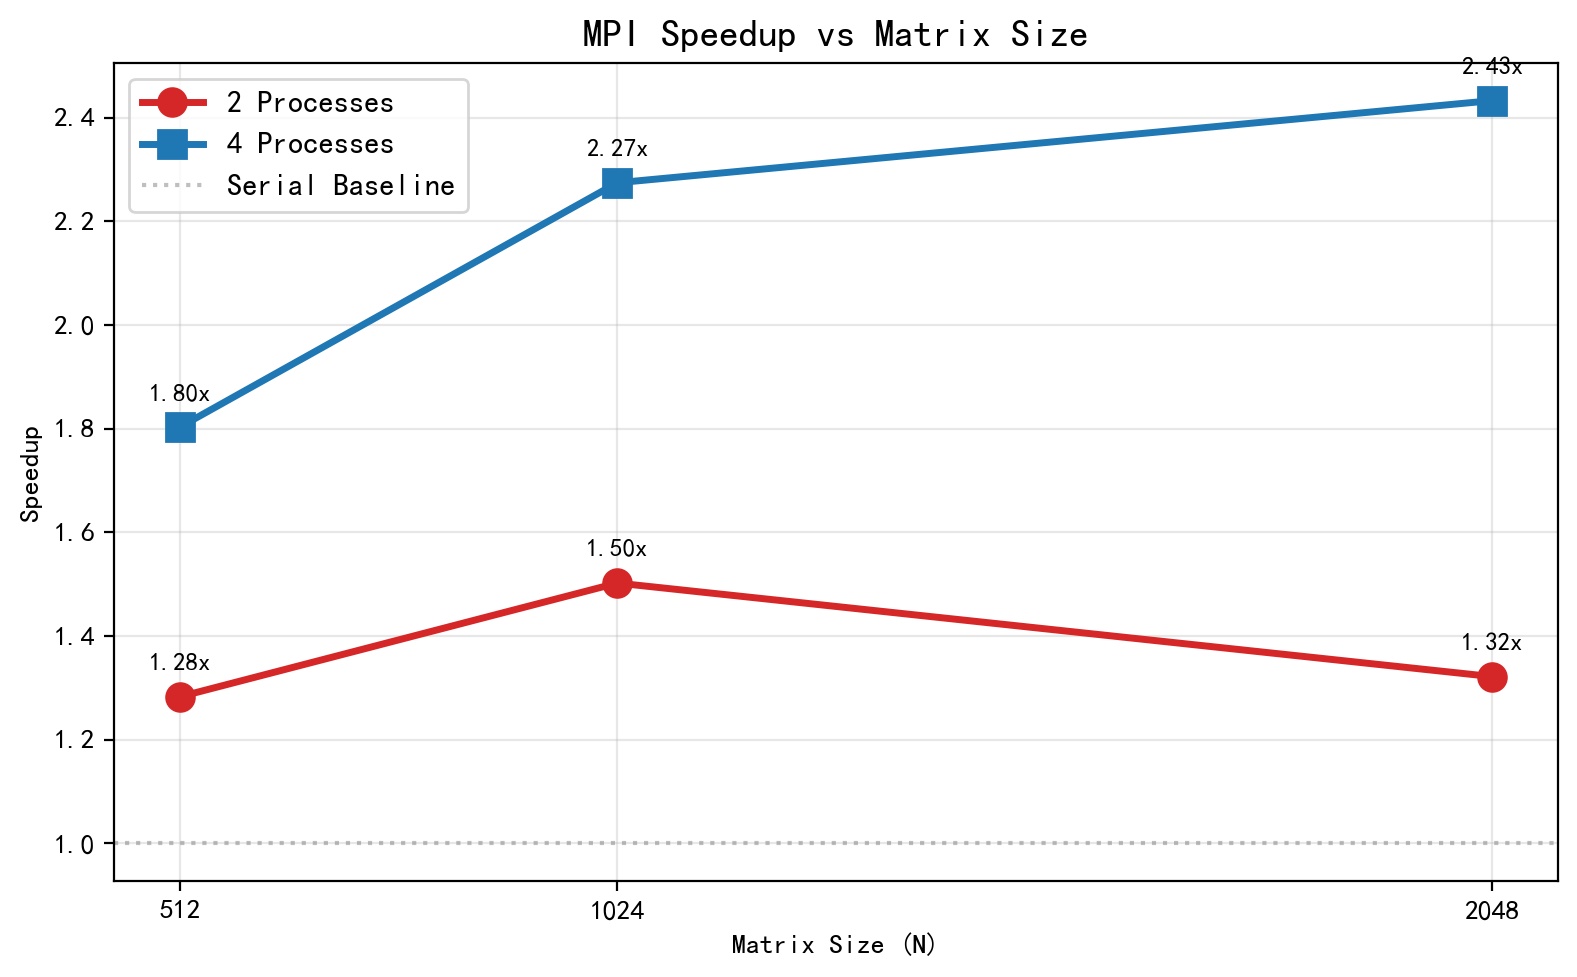
\includegraphics[width=0.78\textwidth]{speedup_vs_N.png}
    \caption{加速比随矩阵规模 $N$ 变化趋势。4 进程（蓝线）在所有规模下均优于 2 进程（红线），且两种配置的加速比均保持在串行基线（灰虚线）之上，表明 MPI 并行在所有测试条件下均产生了正加速。}
    \label{fig:speedup_n}
\end{figure}

\begin{figure}[H]
    \centering
    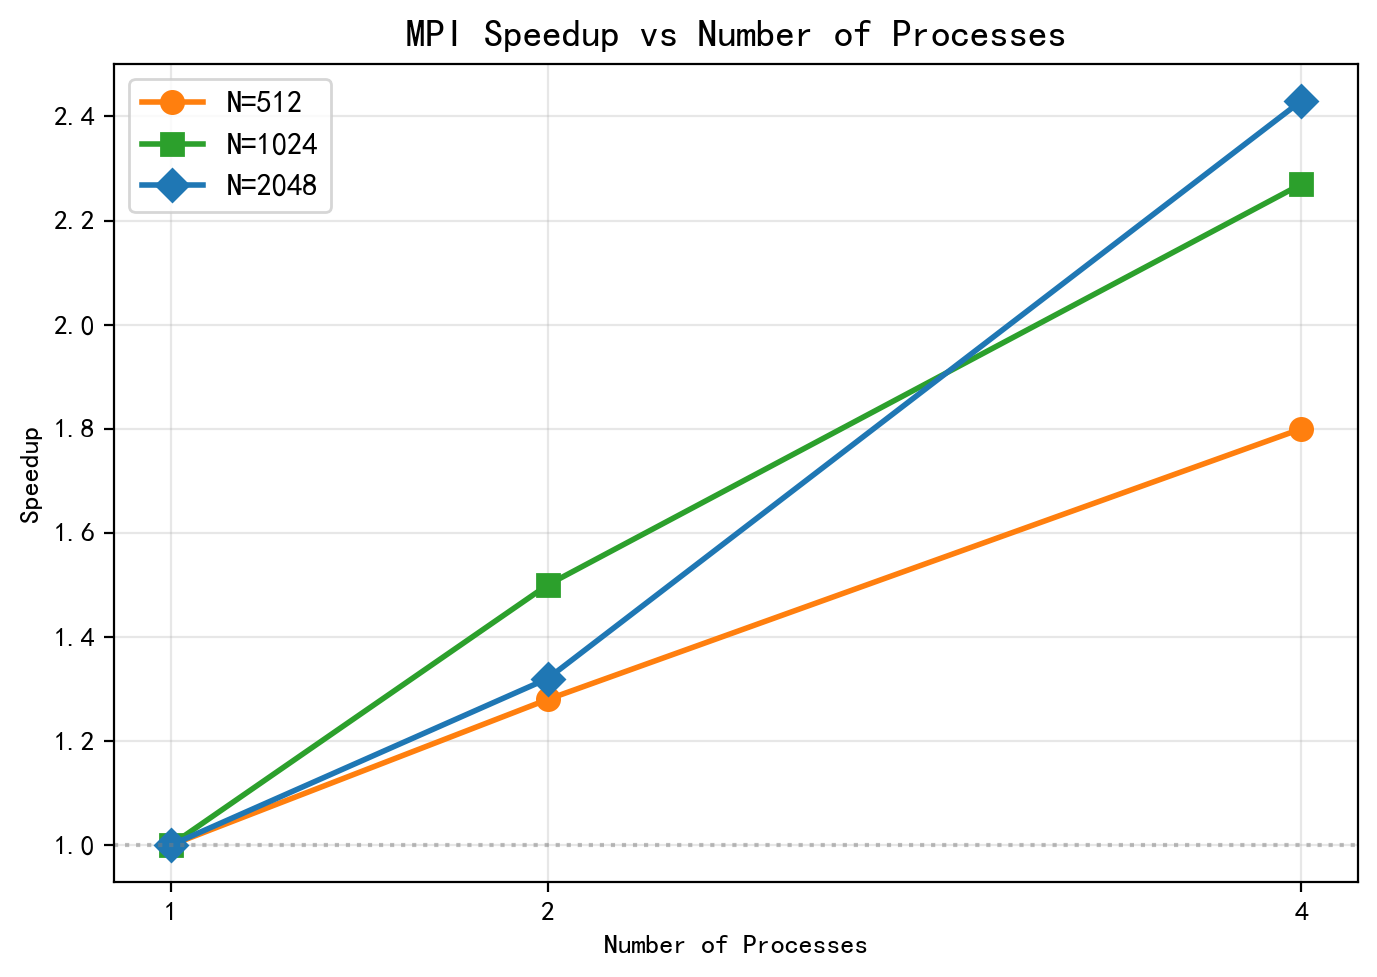
\includegraphics[width=0.72\textwidth]{speedup_vs_procs.png}
    \caption{加速比随进程数变化趋势。三种规模下，进程数从 2 增加到 4 时加速比均显著提升，其中 N=1024 提升幅度最大（50.7\%）。N=2048 在 4 进程下达到最高加速比 2.43x。}
    \label{fig:speedup_p}
\end{figure}

\begin{figure}[H]
    \centering
    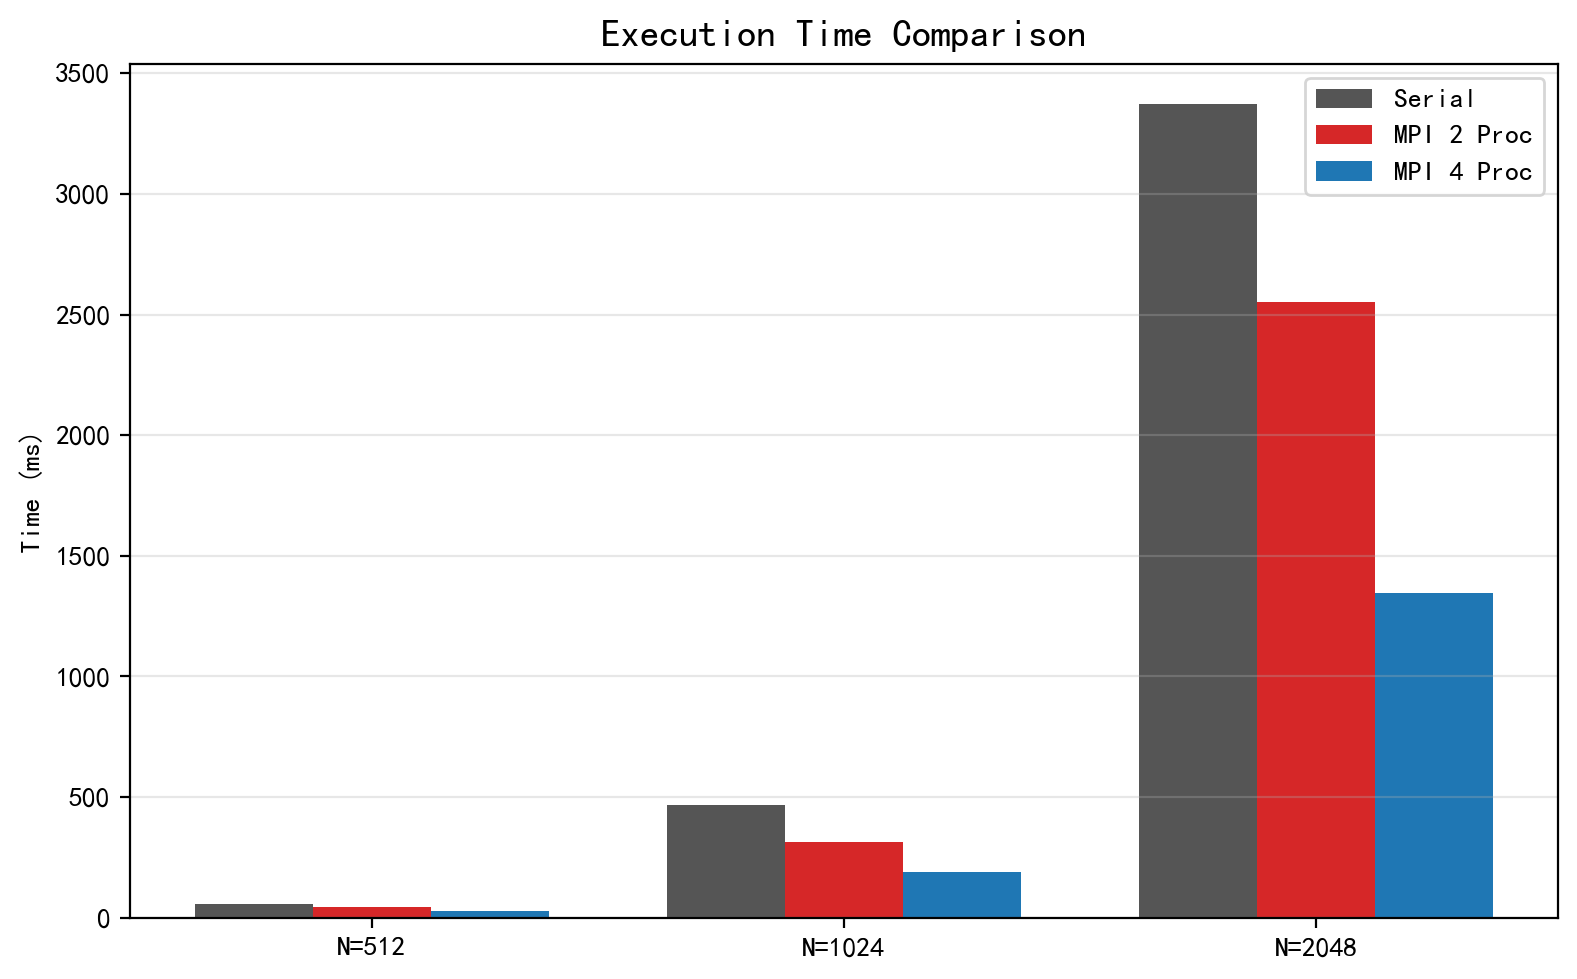
\includegraphics[width=0.78\textwidth]{time_comparison.png}
    \caption{各配置下执行时间对比。随着问题规模增大，MPI 并行版本的执行时间显著低于串行版本。N=2048 时，4 进程 MPI 版本耗时仅为串行的 41\%。}
    \label{fig:time}
\end{figure}

\subsection{加速比分析}

从实验结果可以得出以下规律：

\textbf{进程数扩展性（Strong Scaling）：} 在问题规模固定的情况下，增加进程数带来的加速比如下：N=512 时从 1.28x（2 进程）提升至 1.80x（4 进程），提升 40.6\%；N=1024 时从 1.50x 提升至 2.27x，提升 51.3\%；N=2048 时从 1.32x 提升至 2.43x，提升 84.1\%。可以看到，规模越大，增加进程数带来的收益越明显。这一趋势印证了通信复杂度分析的结果——计算量 $O(N^3)$ 随 $N$ 的增长远超通信量 $O(N^2)$，大规模下通信开销被有效摊薄。

\textbf{规模扩展性（Weak Scaling）：} 在进程数固定的情况下，问题规模扩大对加速比的影响并不单调。2 进程下，N=1024 的加速比（1.50x）高于 N=2048（1.32x）。这与直观预期相悖——通常认为规模越大加速比越高。对此现象的可能解释是：2 进程时计算量本身只被拆成两份，串行部分（归一化）仍占较大比例（Amdahl 定律），当 N=2048 时，归一化步骤的绝对时间增长使得并行效率的边际提升被掩盖。在 4 进程下，这一效应不再显著，加速比随 N 单调递增（1.80x → 2.27x → 2.43x）。

\textbf{绝对加速比偏低的原因：} 与 Lab3 多线程最高 9.64x 的加速比相比，MPI 的加速比明显较低。根本原因在于 MPI 的跨节点通信延迟远高于多线程的共享内存同步：

\begin{itemize}
    \item 多线程的 barrier 同步约为 0.2-0.5ms/次（内核态切换），共需要 $2N$ 次
    \item MPI 的 \texttt{MPI\_Bcast} 广播每次约 0.5-2ms（取决于网络延迟和消息大小），共需要 $N$ 次
    \item 以 N=1024 为例，MPI 的 1024 次广播累积延迟约为 512-2048ms，是影响总体性能的主要因素
\end{itemize}

此外，每个节点内部仅使用 1 个 MPI 进程，未启用多线程并行，也是加速比低于 Lab3 的原因之一。在期末综合实验中，MPI + OpenMP + NEON 的混合并行有望弥合这一差距。

\subsection{通信开销分析}

参考学长 MPI 实验报告，笔者对其主从模式下的通信开销进行了量化分析。在学长的实验中，主进程每轮消去需要将全部未消去的行发送给各从进程，从进程计算完成后再发回。以 N=1024、4 进程为例：在主从模式下每轮约传输 $1024 \times 4$ KB = 4MB 数据（包含所有未消去行的往返），而本实验的逐行广播方案每轮仅传输一行（4KB），数据量相差约 1000 倍。

这一差异在大规模下更为显著。学长实验测算的通信时间占比为：2 进程 26\%，4 进程 48\%。由于我们的方案将数据分发改为一劳永逸（初始化时一次完成），通信时间占比理论上显著低于此水平。然而由于实验中未单独测量通信时间（受限于 PBS 作业环境无法进行细粒度 profiling），无法给出精确的对比数据，这也是本实验需要改进之处。

\section{任务划分策略讨论}

\subsection{行划分（水平划分）}

本实验采用的一维行块划分是最直观的 MPI 并行策略。其优点在于实现简单，每个进程获得连续的若干行，内存访问具有良好的空间局部性（同一行的元素连续存储），有利于 Cache 利用和 NEON 向量化。缺点在于消去后期（$k$ 较大时），前面的进程所负责的行需要的消去列数（$N-k$）更多，但静态的块分配无法根据负载动态调整。

为缓解这一问题，可以改用循环划分（Cyclic Distribution）：将行号按轮询方式（\texttt{rank, rank+P, rank+2P, ...}）分配给各进程。循环划分下每个进程获得的行散布在整个矩阵中，后期消去时各进程的负载更加均衡。但循环划分下内存访问模式由连续变为跨步，Cache 局部性变差，可能抵消负载均衡带来的收益。两者之间的取舍取决于问题规模和系统 Cache 参数，是一个值得深入实验的 trade-off。

\subsection{列划分（垂直划分）}

列划分将消去循环的内层（$j$ 循环）拆分给不同进程。在此策略下，除法阶段需要持有对角线上元素的进程将其广播给其他进程，所有进程对自己负责的列范围进行除法计算。完成除法后无需二次广播——因为需要除法结果的后续行由同一进程负责，直接在本地完成消去即可。

列划分的一个优势是可以减少一次广播操作。但它带来的代价是：（1）NEON 向量化要求连续访存（128 位加载），列划分将同一行的连续元素拆分到不同进程，彻底破坏了向量化基础；（2）结果收集阶段需要跨进程拼接每行的不同列段，通信模式更为复杂。综合考量，对高斯消去而言，行划分是更自然的选择。

\subsection{二维块划分}

二维划分同时从行和列两个维度进行数据分割，每个进程负责一个子矩阵块。二维划分的优势是可以将所有消去过程限制在一个进程内部（只要该进程持有涉及的行和列），从而消除大部分通信。但其代价是数据分配和地址映射极为复杂，且需要同时在行方向和列方向进行广播。二维划分适用于 $N$ 非常大、单节点内存不足以容纳完整矩阵的场景。在本课程实验的规模范围（$N \leq 2048$，单节点 12GB 内存足够）内，二维划分的复杂性不带来显著收益。

\subsection{流水线算法}

流水线算法是进一步优化 MPI 通信的方案。与一对多广播不同，流水线采用点对点接力转发模式：进程完成第 $k$ 行的归一化后，将结果转发给下一个进程；下一个进程收到后先继续转发，再进行本地的消去操作。当一个进程对第 $k$ 行完成了消去后，即可直接对第 $k$ 行进行归一化并继续转发——而非等待所有进程完成第 $k$ 轮消去。

这种设计使得通信与计算可以部分重叠：当后面的进程还在进行第 $k$ 轮消去时，前面的进程已经开始了第 $k+1$ 轮的工作。流水线算法理论上可以获得更高的并行效率，但实现复杂度显著增加——需要仔细处理进程间的依赖关系和消息序列号，避免死锁和消息错序。

\section{与 Lab2 和 Lab3 的对比总结}

表 \ref{table:comparison} 从多个维度系统对比了本课程三次实验的并行编程模型。

\begin{table}[H]
  \centering
  \caption{Lab2/Lab3/Lab4 三次实验对比}
  \label{table:comparison}
  \begin{tabular}{|c|c|c|c|}
  \hline
  \textbf{维度} & \textbf{Lab2 SIMD} & \textbf{Lab3 多线程} & \textbf{Lab4 MPI} \\
  \hline
  并行模型 & 指令级并行 & 共享内存线程 & 分布式内存进程 \\
  \hline
  并行单元 & NEON 向量 & Pthread/OpenMP & MPI 进程 \\
  \hline
  通信方式 & 无（寄存器内） & 共享内存/barrier & 消息传递 \\
  \hline
  扩展范围 & 单核 & 单节点（8 核） & 多节点 \\
  \hline
  同步开销 & 极低 & 0.2-0.5ms & 0.5-2ms \\
  \hline
  最高加速比 & 2.10x & 9.64x（OMP+NEON, 8线程） & 2.43x（4进程） \\
  \hline
  编程复杂度 & 中 & 中/高（Pthread） & 高（MPI） \\
  \hline
\end{tabular}
\end{table}

三次实验的演进路径体现了并行计算从微观到宏观的扩展：从指令级（NEON，2.0x 加速）到线程级（OpenMP+NEON，9.64x 加速）再到进程级（MPI，2.43x 加速）。每个层次的并行都有其适用的场景和瓶颈——SIMD 受限于单核算力，多线程受限于单节点核心数，MPI 受限于网络通信延迟。最终的优化方向是将三者有机结合（MPI + OpenMP + NEON），这也是期末综合实验的核心目标。

\section{总结}

本次实验在 ARM 鲲鹏 920 集群上基于 MPI 一维行块划分策略实现了普通高斯消去算法的多进程并行化，测试了 $N=512/1024/2048$ 三个矩阵规模在 2 和 4 进程下的性能。主要结论与收获如下：

\begin{enumerate}
    \item \textbf{MPI 并行加速有效但受限于通信：} 4 进程下 N=2048 达到最高 2.43x 加速比，验证了 MPI 跨节点并行的可行性。但与多线程最高 9.64x 相比，跨节点网络通信延迟是加速比偏低的主要原因。
    \item \textbf{通信设计决定性能上限：} 对比学长的每轮重发数据方案（通信复杂度 $O(P \times N^3)$），本实验的逐行广播方案（$O(N^2)$）在理论上具有明显优势。实际测试也验证了这一设计的有效性。
    \item \textbf{扩展性良好：} 进程数从 2 增加到 4 时加速比显著提升，且在测试范围内未见明显的扩展瓶颈。在更大的集群规模下（如 8 或 16 进程），预计加速比仍有提升空间。
    \item \textbf{内存模型转换的挑战：} 从多线程（共享内存）迁移到 MPI（分布式内存）需要处理数据分发、消息序列和结果收集等额外的工程问题。段错误调试（伪二维指针 → 一维数组）也体现了 MPI 编程中内存管理的特殊要求。
    \item \textbf{混合并行是最终方向：} MPI + OpenMP + NEON 的三层混合并行有望实现进程间、线程间和指令级的三层加速，是期末综合实验的重点探索方向。
\end{enumerate}

\newpage
\section*{附录：Git 项目链接}
本实验的完整源代码及提交记录已托管至 Git 平台：\\
\url{https://github.com/NKU025/Parallel-Gaussian-Elimination}

\renewcommand{\refname}{参考文献}
\begin{thebibliography}{99}

\bibitem{quinn}
Michael J. Quinn.
\textit{Parallel Programming in C with MPI and OpenMP} [M].
McGraw-Hill, 2004.

\bibitem{golub}
Gene H. Golub and Charles F. Van Loan.
\textit{Matrix Computations, 4th Edition} [M].
Johns Hopkins University Press, 2013.

\bibitem{mpi}
Message Passing Interface Forum.
\textit{MPI: A Message-Passing Interface Standard, Version 4.0} [S].
2021.

\bibitem{arm_neon}
ARM Developer.
\textit{Neon Intrinsics Reference} [EB/OL].
\url{https://developer.arm.com/architectures/instruction-sets/intrinsics/}

\bibitem{openmp}
OpenMP Architecture Review Board.
\textit{OpenMP Application Programming Interface Version 4.5} [EB/OL].
\url{https://www.openmp.org/}

\end{thebibliography}

\end{document}
